%%%%%%%%%%%%%%%%%%%%%%%%%%%%%%%%%%%%%%%%%
% Beamer Presentation
% LaTeX Template
% Version 1.0 (10/11/12)
%
% This template has been downloaded from:
% http://www.LaTeXTemplates.com
%
% License:

% CC BY-NC-SA 3.0 (http://creativecommons.org/licenses/by-nc-sa/3.0/)
%
%%%%%%%%%%%%%%%%%%%%%%%%%%%%%%%%%%%%%%%%%

%----------------------------------------------------------------------------------------
%	PACKAGES AND THEMES
%----------------------------------------------------------------------------------------

%\documentclass{beamer}

\documentclass[handout]{beamer}

\mode<presentation> {

% The Beamer class comes with a number of default slide themes
% which change the colors and layouts of slides. Below this is a list
% of all the themes, uncomment each in turn to see what they look like.

\usetheme{default}
%\usetheme{AnnArbor}
%\usetheme{Antibes}
%\usetheme{Bergen}
%\usetheme{Berkeley}
%\usetheme{Berlin}
%\usetheme{Boadilla}
%\usetheme{CambridgeUS}
%\usetheme{Copenhagen}
%\usetheme{Darmstadt}
%\usetheme{Dresden}
%\usetheme{Frankfurt}
%\usetheme{Goettingen}
%\usetheme{Hannover}
%\usetheme{Ilmenau}
%\usetheme{JuanLesPins}
%\usetheme{Luebeck}
\usetheme{Madrid}
%\usetheme{Malmoe}
%\usetheme{Marburg}
%\usetheme{Montpellier}
%\usetheme{PaloAlto}
%\usetheme{Pittsburgh}
%\usetheme{Rochester}
%\usetheme{Singapore}
%\usetheme{Szeged}
%\usetheme{Warsaw}

% As well as themes, the Beamer class has a number of color themes
% for any slide theme. Uncomment each of these in turn to see how it
% changes the colors of your current slide theme.

%\usecolortheme{albatross}
%\usecolortheme{beaver}
%\usecolortheme{beetle}
%\usecolortheme{crane}
%\usecolortheme{dolphin}
%\usecolortheme{dove}
%\usecolortheme{fly}
%\usecolortheme{lily}
%\usecolortheme{orchid}
%\usecolortheme{rose}
%\usecolortheme{seagull}
\usecolortheme{seahorse}
%\usecolortheme{whale}
%\usecolortheme{wolverine}

\setbeamertemplate{footline} % To remove the footer line in all slides uncomment this line
%\setbeamertemplate{footline}[page number] % To replace the footer line in all slides with a simple slide count uncomment this line

\makeatletter
\setbeamertemplate{footline}
{
  \leavevmode%
  \hbox{%
  \begin{beamercolorbox}[wd=.333333\paperwidth,ht=3.2ex,dp=1ex,center]{author in head/foot}%
    \usebeamerfont{author in head/foot}\insertsection
  \end{beamercolorbox}%
  \begin{beamercolorbox}[wd=.333333\paperwidth,ht=3.2ex,dp=1ex,center]{title in head/foot}%
    \usebeamerfont{title in head/foot}\insertsubsection
  \end{beamercolorbox}%
  \begin{beamercolorbox}[wd=.333333\paperwidth,ht=3.2ex,dp=1ex,right]{date in head/foot}%
    \usebeamerfont{date in head/foot}\insertauthor \,  Ph.D. defense \hspace*{2em}
  \end{beamercolorbox}}%
  \vskip0pt%
}
\makeatother

%\setbeamertemplate{navigation symbols}{} % To remove the navigation symbols from the bottom of all slides uncomment this line
}
\addtobeamertemplate{navigation symbols}{}{%
    \usebeamerfont{footline}%
    \usebeamercolor[fg]{footline}%
    \hspace{1em}%
    \insertframenumber/\inserttotalframenumber
}

\newcommand*{\mathcolor}{}
\def\mathcolor#1#{\mathcoloraux{#1}}
\newcommand*{\mathcoloraux}[3]{%
  \protect\leavevmode
  \begingroup
    \color#1{#2}#3%
  \endgroup
}
\newcommand{\fc}{\mathfrak{c}}



\usepackage{macros}
\usepackage{color}
\usepackage{algpseudocode}
\usepackage{algorithmicx}
\usepackage{algorithm}
\usepackage{physics}
\renewcommand{\algorithmicrequire}{\textbf{Input:}}
\renewcommand{\algorithmicensure}{\textbf{Output:}}

%\usepackage{handoutWithNotes}
%\pgfpagesuselayout{3 on 1 with notes}[a4paper, border shrink=5mm]
\usepackage{tikz-cd}

%\usepackage{graphicx} % Allows including images
\usepackage{booktabs} % Allows the use of \toprule, \midrule and \bottomrule in tables
%----------------------------------------------------------------------------------------
%	TITLE PAGE
%----------------------------------------------------------------------------------------

\DeclareMathOperator{\cond}{cond}

\title[thesis defense]{Computational aspects of modular parametrizations \\ of elliptic curves} % The short title appears at the bottom of every slide, the full title is only on the title page

\author{Hao Chen} % Your name
\institute[UW] % Your institution as it will appear on the bottom of every slide, may be shorthand to save space
{
University of Washington Ph.D. defense \\ % Your institution for the title page
\medskip
Advisor: William Stein % Your email address
}
\date{April 26, 2016} % Date, can be changed to a custom date

\begin{document}

\begin{frame}
\titlepage % Print the title page as the first slide
\end{frame}


%
%\begin{frame}
%\frametitle{Overview} % Table of contents slide, comment this block out to remove it
%\huge \tableofcontents[hideallsubsections] % Throughout your presentation, if you choose to use \section{} and \subsection{} commands, these will automatically be printed on this slide as an overview of your presentation
%\end{frame}

%----------------------------------------------------------------------------------------
%	PRESENTATION SLIDES
%----------------------------------------------------------------------------------------

%\begin{frame}
%\tableofcontents
%\end{frame}

%------------------------------------------------
\section{Critical subgroups of elliptic curves} % Sections can be created in order to organize your presentation into discrete blocks, all sections and subsections are automatically printed in the table of contents as an overview of the talk
%------------------------------------------------

% A subsection can be created just before a set of slides with a common theme to further break down your presentation into chunks
 \begin{frame}
 \frametitle{\insertsection}
 \tableofcontents[currentsection]
 \end{frame}

%-------------
\subsection{Elliptic curves and modular curves}

\begin{frame}
\frametitle{Elliptic curves over $\bQ$}
\begin{Def}
An \red{elliptic curve} over $\bQ$ is a nonsingular projective curve $E \subseteq \bP^2$ with defining equation 
\begin{equation*}
y^2z = x^3 + Axz^2+Bz^3, 
\end{equation*}
where $A,B \in \bQ$ and  $4A^3+27B^2 \neq 0$.
\end{Def}

% The {\bf invariant differential}:  $\omega_E = \frac{dx}{y}$.

%$E(\bC)$ is a Riemann surface of genus 1, which is topologically a torus. % $E(\bQ)$ = The subgroup of rational solutions to \ref{eq:1}.

\pause

\begin{theorem}[Mordell-Weil]
$E(\bQ)$ is a finitely generated abelian group, i.e., $$E(\bQ) \cong \bZ^r \oplus T,$$
for some $r \geq 0$ and $T$ finite. 
\end{theorem}
$r$ is called the \red{rank}. $T$ is the \red{torsion subgroup}. 

\end{frame}

%\begin{frame}
%\frametitle{Group law on elliptic curves(I)}
%\centering
%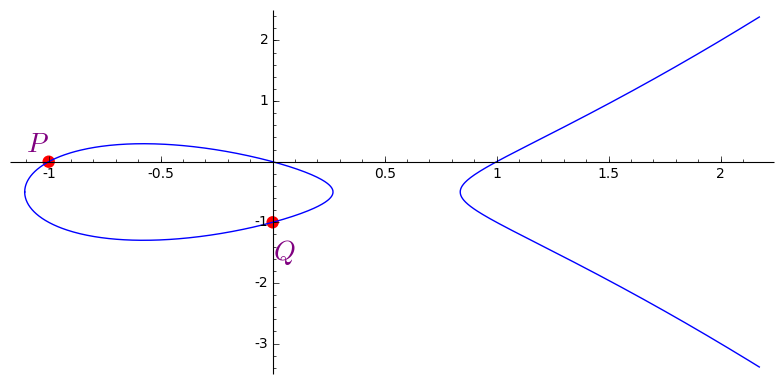
\includegraphics[width=0.8\linewidth]{pics/1.png}
%\end{frame}

%\begin{frame}
%\frametitle{Group law on elliptic curves(II)}
%\centering
%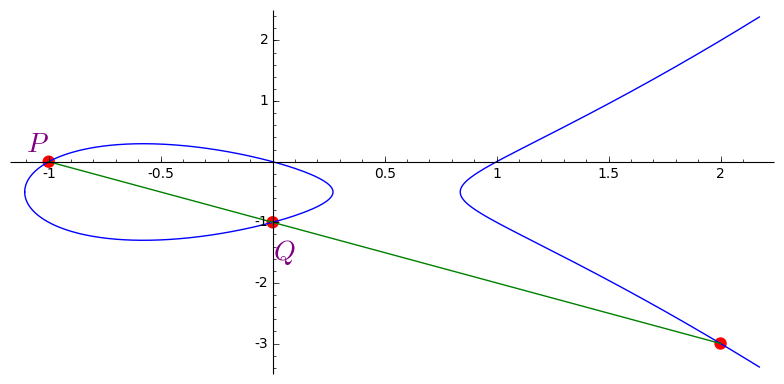
\includegraphics[width=0.8\linewidth]{pics/2.png}
%\end{frame}

\begin{frame}
\frametitle{The BSD conjecture} 


% $rank(E(\bQ))$ has been studied extensively in number theory. \\ % up to now, no easy way of computing the rank.
There is an entire function $L(E,s)$ called the $L$-function of $E$.  \\

\medskip
\pause

The rank part of the  \red{Birch and Swinnerton-Dyer (BSD) conjecture} is
\begin{equation*}
	rank(E(\bQ)) = \ord_{s=1}L(E,s).
\end{equation*}

\pause
\medskip

\begin{itemize}
\item $\ord_{s=1}L(E,s)$ is called the analytic rank, denoted by \red{$r_{an}(E)$}. \\
\item The BSD conjecture is open when $r_{an}(E) > 1$. \\
\item The proof of rank BSD for $r_{an}(E) \leq 1$ uses Heegner points. 
\end{itemize}

\end{frame}


%------------------------------------------------

\begin{frame}
\frametitle{Modular curves}
Let $N \geq 1$ be an integer, consider the group 
\[
	\Gamma_0(N) = \left \{ \abcd{a}{b}{c}{d} \in SL_2(\bZ): N \mid c \right\}.
\]
Let $\cH^* := \{z \in \bC: im(z) > 0\} \cup \bQ \cup \infty$.  $\Gamma_0(N)$ acts on $\cH^{*}$. 

\begin{Def}
$X_0(N) = \Gamma_0(N) \backslash \cH^*$ is the \red{modular curve} of level $N$. 
\end{Def}

\begin{itemize}
\item $X_0(N)$ is a  nonsingular projective curve.
%\item Rational functions on $X_0(N)$ have \red{$q$-expansions} at infinity:
%\[
%	u(q)  = \sum_{n \geq -m} b_n q^n, \; q = e^{2 \pi i z}. 
%\]
\end{itemize}
\end{frame}

\begin{frame}
\frametitle{The modularity theorem}
%Notation: for a cusp form f weight 2 and level $N$, let $\omega = f(z)dz$.

%\begin{Fact}
%$\omega$ is a holomorphic differential on $X_0(N)$.
%\end{Fact}

The \red{Modularity Theorem} (Breuil, Conrad, Diamond, Taylor) proves the existence of an integer $N > 1$ and a surjective morphism 
$\varphi: X_0(N) \to E$ defined over $\bQ$.

\pause
\medskip

The smallest such $N$ is called the conductor of $E$. 

\pause
\medskip

Let $\omega = \varphi^*(\frac{dx}{y})$. Then $$\omega = c f(z) \mathrm{d} z$$ where $f$ is the \red{modular form attached 
to $E$}.  \\

\smallskip

We assume $E$ is optimal. Then $\varphi$ is unique up to sign.


\end{frame}
\begin{frame}

Idea: use $\varphi$ to find rational points on $E$ from special points on $X_0(N)$. 

\begin{itemize}
\item rational points on $X_0(N)$ -- usually get torsion points.  
\item Heegner points.  -- Great for $r_{an}(E) = 1$. Always torsion when $r_{an}(E) \geq 2$.
\item Ramification points -- probably always torsion when $r_{an}(E)$ is even. 
\item Others?? 
\end{itemize}

Note: up to now, no known construction in $\geq 2$. 


\end{frame}

% Note: the elliptic points, when they exist, are Heegner points on $X_0(N)$.

% nothing to do with level.
%From the Gross-Zagier formula, we can derive:

\subsection{The critical subgroup and critical polynomials}

\begin{frame}{The critical subgroup $E_{crit}(\bQ)$}
%\frametitle{Background: Ramification}

%Given any morphism $\varphi: X \to Y$ between curves, the ramification divisor of $\varphi$ is 
%\[
%	R_\varphi = \sum_{x \in X} (e_\varphi(x) - 1) [x]
%\]
%there is a finite set of points $x \in X$ where 
%the preimage $\varphi^{-1}(\varphi(x))$ is `smaller than usual'. Such x is called a {\bf critical point}, 
%and $f(x)$ is called a ramification point. 
%For example, the projection $\{(x,y) \in \bR^2: x = y^2\} \to \bR: (x,y) \mapsto x$ 
%is ramified at $(0,0)$.

%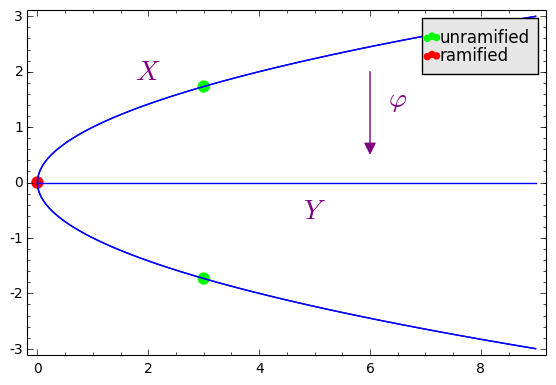
\includegraphics[width=10cm,height=7cm]{pics/ramification.png}


%\end{frame}

%\begin{frame}{Riemann-Hurwitz Formula}
%Some of on divisors: 
%\begin{itemize}
%\item A {\bf divisor} $D$ on a curve $X$ is a finite formal sum of points $D = \sum_{x \in X} n_x[x]$, $n_x \in \bZ$.\\
%\item $\supp D = \{x: n_x \neq 0\}$ = the {\bf support} of the divisor. 
%\item For $f \in \bQ(X)$, $\Div(f) = \{\mbox{zeros of } f\} - \{\mbox{poles of } f\}$.
%\item Divisor of differentials are defined similarly. 
%\end{itemize}

%For every $\varphi: X \to Y$, there exists a divisor $R_{\varphi} \geq 0$, called 
%the \textbf{ramification divisor} of $\varphi$, such that 
%$\supp R_{\varphi} = \mbox{ critical points of } \varphi$.

%\begin{theorem}[Riemann-Hurwitz formula]
%If $\varphi: X \to Y$ is a non-constant morphism of curves and $\omega$ is any differential on $X$, then 
%\[
%          \Div(\varphi^*(\omega))   = \varphi^*(\Div(\omega)) + R_{\varphi}.
%\]
%\end{theorem}
% Let $\varphi: X_0(N) \to E$ be the modular parametrisation and let 

Observation: if $K$ is a number field and  $P \in E(K)$, then we can ``trace down to $\bQ$''. That is, 
The point $tr(P) := \sum_{\sigma: \bQ(P) \to \bar{\bQ}} P^{\sigma}$ is in $E(\bQ)$. 

\pause 
\medskip

\begin{Def}[Mazur, Swinnerton-Dyer]
The \red{critical subgroup} of $E$, denoted by $E_{crit}(\bQ)$, is the group generated by traces of 
images of ramification points of $\varphi$.  
\end{Def}

\pause
%Riemann-Hurwitz formula + $\Div(\omega_E) = 0$  $\implies .
%(a canonical divisor on $X_0(N)$). \\

%$\varphi$ is ramified at $2g-2$ points, counting  multiplicity.
%  F.Brunault: a sufficient condition such that $R_\varphi$ 
%does not contain cusps

\begin{question}[Mazur and Swinnerton-Dyer, 1974]
Is there an elliptic curve $E/\bQ$ with $r_{an}(E) \geq 2$ and $rank(E_{crit}(\bQ)) >0$?
\end{question}
\end{frame}


\begin{frame}

\begin{theorem}[C.]
For all elliptic curves $E$ of rank 2 and conductor $N <1000$, the rank of $E_{crit}(\bQ)$ is 0.
\end{theorem}

To prove this, we compute $E_{crit}(\bQ)$ for each curve. 

 % Then he uses a complex form of modular parametrisation to compute $E_{crit}(\bQ)$.

\end{frame}

%------------------------------------------------





\begin{frame}{Critical $j$-polynomial}
%The group $E(\bQ)$ has been studied extensively in number theory.
%Associated to $E$ is an analytic function $L(E,s)$( the L-function of E). \\
%The rank part of the B-SD conjecture states
%\[
%	rank(E(\bQ)) = \ord_{s=1}L(E,s).
%\] 
%It is proved for $\ord_{s=1}L(E,s) \leq 1$.


%\end{frame}

%\subsection{Critical Polynomial}
%\begin{frame}
%\frametitle{Critical Polynomials}

%Notation: $Z_\omega =$.  \\

To help compute $E_{crit}(\bQ)$, we make the following definition. 
\begin{Def}
%Let $E/\bQ$ be an elliptic curve of conductor $N$ and let $j$ be the $j$-invariant. 
The \red{critical j-polynomial} of $E$ is 
\[
F_{E,j}(x) = \prod_{z \in Y_0(N)}(x-j(z))^{mult_{Ram(\varphi)}(z)}.
\]
\end{Def}
We have $F_{E,j}(x) \in \bQ[x]$ and $\deg F_{E,j} \leq 2g-2$.  

\pause
\medskip

For $h \in \bQ(X_0(N))$, can define $F_{E,h}(x)$. 

\pause
\medskip


\begin{Example}
$F_{{\bf 44a},j}(x) = H_{-44}(x)^2$. $F_{{\bf 37a},j}(x) = H_{-148}(x)$. $F_{{\bf 37b},j}(x) = H_{-16}(x)^2$.
\end{Example}
Here $H_d$ is the Hilbert class polynomial of disc $d$. 


\end{frame}

%------------------------------------------------

\begin{frame}{Computing $F_{E,j}$}
%When  $N$ is not square free, \textbf{NORM} does not work. \textbf{IPR} is an algorithm to compute $F_{E,j}$, which works for any $N$. \\
Idea: use the fact that $Ram(\varphi) = Div(\omega)$. Take two rational functions 
$r := (j-1728)  \frac{\omega}{{d j}}, \;  u := \frac{1}{j}$ on $X_0(N)$. 


%Moreover, if $T >  2g-2$, then the pair $(rj^T,u)$ satisfies the conditions of the proposition. (\hyperlink{condition is satisfied}{\underline{One proves it by looking at the zeros and poles of $rj^T$}}). % Proof is not long, but please believe me. t

\begin{Prop}[C.]
For $T \gg 0$, let $P(x,y) = f_n(y)x^n + \cdots + f_1(y)x + f_0(y)$ be an irreducible polynomial over $\bQ$,  such that $P(u, rj^T) = 0$.  Then
\[
		F_{E,j}(x) = P(\frac{1}{x}, 0) \cdot x^{A} (x - 1728)^B
\]	
where $A,B$ are explicitly computable. 
\end{Prop}

Hence,  it suffices to compute the polynomial $P$, which can be done using \red{linear algebra}, given the 
$q$-expansions of $r$ and $u$. 

\end{frame}


%\begin{frame}{More examples of critical $j$-polynomials computed via the {\bf IPR} algorithm}
%\begin{Example}
%$E = \textbf{197a}$, we obtain
%\[
%	F_{E,j}(x)  = (x + 884736)^2 H_{-197 \cdot 4}(x) f_{18}(x),
%\]
%where $f_{18}$ is an irreducible polynomial in $\bQ[x]$ of degree 18.
%\end{Example}

%\begin{Example}
%\label{ex: 389a}
%$E = \textbf{389a}$, the curve of algebraic rank 2 with smallest conductor. 
%\[
%	F_{E,j}(x)  = (x + 884736)^2 f_{60}, 
%\]
%where $f_{60}$ is irreducible of degree 60. 
%This example will be revisited in Section ~\ref{sec:exact points}. 
%\end{Example}

%\pause



% \hyperlink{yang pair}{Yang pair}


%\end{frame}

%------------------------------------------------

%\begin{frame}{Integer Polynomial Relation(IPR): Example}
%\begin{Example}
%$E = \textbf{44a}$,
%\begin{align*}
%F_{E,j}(x) &= (x^{3} - 1122662608x^{2} + 270413882112x - 653249011576832)^2  \\
%            &= H_{-44}(x)^2.
%\end{align*}
%\end{Example}

%\begin{Example}
%$E = \textbf{48a}$, $F_{E,j}(x) = 1$. Explanation: All critical points are cusps. In fact, $Z_{\omega}  = [1/4] + [3/4] + [1/12] +[7/12]$. 
%\end{Example}


%\end{frame}


%------------------------------------------------
%\section{Algorithm: Yang pair}

%\begin{figure}
%\includegraphics[width=0.8\linewidth]{test}
%\end{figure}


%------------------------------------------------

%Remark: once we have $F(r_1, h_2) = 0$, let $F_0(x) = F(0,h_2)$. Then $F_{E,h} =  F(0,h_2)/(*)$, where $(*)$ the extra factor  coming from zeros of $h_1$. $(*)$ is explicitly computable, but we may also `eyeball' it. \\




%------------------------------------------------
\subsection{Computing the critical subgroup}

\begin{frame}{The critical subgroup $E_{crit}(\bQ)$}

% Recall the definition: $E_{crit}(\bQ) = \langle tr(\varphi(e)): e \in \supp \Div(\omega)\rangle$. We observe that 

%Write $Z_\omega = \sum_{i = 1}^n n_i S_i$, where the $n_i \in \bZ_{\geq 1}$ and each $S_i$ is a sum of points in a Galois orbit. Set $P_i = \sum \varphi_*(S_i) \in E(\bQ)$. Let $E_{crit}^u(\bQ)  = \langle \{P_i\}_i \rangle$.
%\begin{Lemma}
%$E_{crit}(\bQ) \otimes \bQ = E_{crit}^u(\bQ) \otimes \bQ$, i.e., $E_{crit}^u(\bQ)$ and  $E_{crit}(\bQ)$ have the same rank as abelian groups.
%\end{Lemma}


%\begin{itemize}
%\item Observation: $g = \frac{f\Delta}{E_4^2E_6} \in \bQ(X_0(N))$.  \\
%\item Therefore, $\varphi_*(\Div(g)) = \Div(\varphi_*(g))$(i.e., it is a principal divisor). \\
%\item However, if $D = \sum n_P[P]$ is a principal divisor on $E$, then $\sum n_P P = 0 \in E(\bQ)$. \\
%\item This gives a linear relation on the images of zeros of these four modular forms. 
%\end{itemize}
%\begin{align*}
%& \implies \varphi_*(\Div(g)) = 0 \in Div^0(E) \\
%& \implies \sum_{z \in \Div(g)} n_z\varphi(z) = 0 \in E(\bQ). 
%\end{align*}

%Recall the lemma: 
%\begin{Lemma}[C.]
%$6 P_{all} =  - 3 \sum_{c \in Ell_2(N)} \varphi(c) - 4 \sum_{d \in Ell_3(N)} \varphi(d)$. \\
%\end{Lemma}

% If $r_{an}(E) \geq 2$, then the right hand side is torsion by Gross-Zagier, hence

%\begin{Prop}[C.]
%Assume either $r_{an}(E) \geq 2$ or $X_0(N)$ has no elliptic point. Then $P_{all} \in E(\bQ)_{tors}$,  hence $rank(E_{crit}(\bQ)) \leq n_{\omega} - 1$. 
%\end{Prop}
%\pause

%If in addition $r_{an}(E)$ is even, then $w_N(\varphi(e)) \equiv - \varphi(e) \pmod {E(\bar{\bQ)}_{tors}}$ for all $e \in X_0(N)$.
\begin{Theorem}[C.]
\label{cor: cm}
%Let $E/\bQ$ be an elliptic curve of conductor $N$. 
Suppose the analytic rank of $E$ is at least 2, and assume at least one of the following holds: \\ 
\vspace{4mm}
(1) $F_{E,j} = \prod_{m =1}^k H_{D_m}^{s_i}\cdot F_0$, where 
$\bQ(\sqrt{D_m}) \neq \bQ(\sqrt{D_n})$ for all $m\neq n$, and $F_0$ is irreducible. \\
(2) $F_{E,h}$ is irreducible for some non-constant function $h \in \bQ(X_0(N))$. \\

\vspace{4mm}

Then $rank(E_{crit}(\bQ))  = 0$.   In other words, the critical subgroup does not contain points of infinite order.
\end{Theorem}
\end{frame}


%------------------------------------------------

\begin{frame}
\frametitle{Critical polynomials for elliptic curves of rank 2 and conductor $<1000$ (I)}
\begin{center}
   \begin{table}[h!]
    \begin{tabular}{ | l | l | l | |p{4.4cm}  |}
    \hline
    $E$ & $g(X_0(N))$    & $h$ & $\mbox{ Factorization of } F_{E,h}(x)$     \\ \hline \hline
    389a & 32  & $j$ & $H_{-19}(x)^2 (x^{60}+ \cdots)$ \\ \hline
    433a & 35  & $j$ &  $x^{68}+\cdots$  \\ \hline
     446d & 55  & $j$ &  $x^{108}+\cdots$ \\ \hline
    563a & 47  & $j$ &  $H_{-43}(x)^2 (x^{90} - \cdots)$   \\ \hline
    571b& 47  & $j$ &  $H_{-67}(x)^2 (x^{90} - \cdots)$ \\ \hline
    643a& 53  & $j$ &  $H_{-19}(x)^2 (x^{102} - \cdots)$ \\ \hline
    664a & 81    &   $\frac{\eta_4\eta_8^2 \eta_{332}^5}{\eta_{166}\eta_{664}^{6}{\eta_2}}$ & $x^{160} - \cdots$ \\ \hline
    655a& 65  & $j$ &  $x^{128} - \cdots$ \\  \hline
    681c& 75  & $j$ &  $x^{148} - \cdots$ \\  \hline
    707a & 67  & $j$ & $x^{132} - \cdots$ 
        \end{tabular}
    \label{table: rank two}	
   \end{table}
\end{center}


\end{frame}
 

\begin{frame}
\frametitle{Critical polynomials for elliptic curves of rank 2 and conductor $<1000$ (II)}   \begin{table}[h!]
    \begin{tabular}{ | l | l | l |p{4.4cm} |}
    \hline
    $E$ & $g(X_0(N))$    & $h$ & $\mbox{ Factorization of } F_{E,h}(x)$     \\ \hline \hline
    709a& 58  & $j$ &  $x^{114} - \cdots$\\ \hline
    718b& 89  & $j$ &  $ H_{-52}(x)^2 (x^{172} - \cdots)$\\ \hline
    794a& 98  & $j$ &  $H_{-4}(x)^2 (x^{192} - \cdots)$\\ \hline
    817a& 71  & $j$ &  $x^{140} - \cdots$\\ \hline
    
    916c & 113   & $j$ &$H_{-12}(x)^8(x^{216}+\cdots)$  \\ \hline
    
   % 916c & 113   & $\frac{\eta_2^7  \eta_{458}^5}{\eta_{229}\eta_{916}^6\eta_4^2 \eta_1^3}$ &\footnotemark $(x^2 - 28x + 3664)^2(x^2 + 116x + 3664)^2(x^{216}+\cdots)$  \\ \hline
    
    944e & 115    & $\frac{\eta_{16}^4 \eta_{4}^2}{\eta_8^6}$ & $x^{224} - \cdots$.\footnotemark \\ \hline 
    997b& 82  & $j$ &  $H_{-27}(x)^2 (x^{160} - \cdots)$\\ \hline
    997c& 82  & $j$ &  $x^{162} - \cdots$\\ \hline
    \end{tabular}
    \label{table: rank two}	
   \end{table}
   	\footnotetext[1]{Here 4 of the critical points are cusps, so $\deg F = 2g- 6$.}
\end{frame}

%------------------------------------------------


%All critical $j$-polynomials in the table are of the form $F_{E,j} = f_{CM}f_0$, so $E_{crit}(\bQ)$ is torsion in these cases. \\
%The critical $h$-polynomial for the curves \textbf{664a} and \textbf{994e} are irreducible, hence $E_{crit}(\bQ)$ is torsion for these two curves. \\ 
%The critical $h$-polynomial for the curve \textbf{916c} is not irreducible, but...\\
%the two quadratic factors in its factorisation correspond to CM points on $X_0(N)$ with j-value 54000. Therefore, $E_{crit}(\bQ)$ is torsion as well.  \\

\begin{frame}{Discussion}

\pause
\smallskip
Future work: 
\begin{itemize}
\item Compute $E_{crit}(\bQ)$ for $E = {\bf 5077a}$. 

Current method will take roughly  5500 hours (parallel computation using 64 cpus). 

\item Prove there are infinitely many elliptic curves with rank  2 such that the critical subgroup is 
torsion.
\end{itemize}

\end{frame}



% Extra slides that I may not need.
%----------------------------------------------------------------------------------------



% modular forms
%----------------------------------------------------------------------------------------

\section{$q$-expansion of newforms at all cusps} 

 \begin{frame}
 \frametitle{\insertsection}
Why study $q$-expansion of newforms at all cusps? (The theory of expansion at the cusp $\infty$
is well known).

\pause 

\begin{itemize}
\item It gives a direct way to compute the critical subgroup. 
\item It gives information about the ramification of $\varphi$ at cusps. 
\item It is useful in computing the Galois representation attached to modular forms. 
\end{itemize}

\end{frame}


\subsection{Problem description}



\begin{frame}
\frametitle{Modular forms}
Let $f$ be a function $f: \cH \to \bC$,  $\alpha  = \abcd{a}{b}{c}{d} \in SL_2(\bZ)$, and let $k \in \bZ$. The weight-k action of $\alpha$ on $f$ is
defined by
\[
	f|[\alpha]_k(z) := (cz+d)^{-k}f(\alpha z).
\]

\pause

\begin{Def}
A \textbf{modular form} of weight $k$ and level $N$ is a holomorphic function $f: \cH \to \bC$ s.t. \\
(1) $f(z)  = f|[\alpha]_k(z), \; \forall \alpha \in \Gamma_0(N)$ ($\Gamma_1(N)$). \\
(2) $f$ has holomorphic extension to all cusps of $X_0(N)$ ($X_1(N)$). \\
\end{Def}

\pause

\red{Cusp forms} = modular forms that are zero at all cusps. \\
Modular forms have \red{$q$-expansions}: $f(q) = \sum_{n \geq 0} a_n q^n$, $q = exp(2\pi i z)$. \\

\end{frame}


\begin{frame}{Newforms and Twists}

Let $S_k(N)$ denote the space of cusp forms. 

\begin{itemize}
\item $S_k(N)$ decomposes in to a direct sum of the old subspace and the new subspace. 
\item The new subspace has a basis of simultaneous eigenforms for certain operators (Hecke operators). 
These eigenforms are called \red{newforms}.
\end{itemize}

Also,  modular forms attached to elliptic curves over $\bQ$ are newforms.  \\ 
We will focus on newforms from now. 
\end{frame}





\begin{frame}{Fourier expansion}
Let $f \in S_k(\Gamma_0(N))$ be a newform and let $\fc = [\frac{a}{c}] \in X_0(N)$ be a cusp. \\


Goal: compute the expansion of $f$ at $\fc$. Denote the expansion by $f_{\fc}(q)$.  \\

\begin{theorem}[C.]
Let $c' = \frac{N}{c}$. Then 
\begin{equation*} \label{expansion0}
f_{[\frac{a}{c}]} \left( q\right) = \frac{w(f) }{\varphi(c')}\sum_{\chi: \cond(\chi) \mid c'} \chi(-a) R(f,\chi)(q)
\end{equation*}

\end{theorem}
Here $R(f, \chi)(q)$ is certain power series in $q$, and it can be computed knowing the \red{twist} $f \otimes \chi$ and the \red{pseudo-eigenvalue} $w(f \otimes \chi)$. 



\end{frame}

\iffalse
\begin{frame}{Idea of computing}

Let $S_c' = \abcd{1}{\frac{1}{c'}}{0}{1}$ and $A_c' = \abcd{1}{0}{c'}{1}$.  Then 
\[
	A_c^{-u} = W_N S_{c'}^u W_N, \, \forall u \in \bZ. 
\]
For a character $\chi$ modulo $c'$, put 

$f|R_\chi(\cond \chi) = g(\bar{\chi})f_\chi$. ($f_\chi (q) = \sum a_n(f) \chi(n)  q^n$ is a modular form of level $N'$.)   We have \begin{equation} 
\label{formula}
	\varphi(c') A_c^{-a} = \sum_{\cond(\chi) \mid c'} \chi(a) W_N R_\chi(c') W_N. 
\end{equation}

Applying to $f$, we arrive at

\end{frame}
\fi



\begin{frame}{Examples (I)}

\begin{Example}
Let $E = {\bf 50a}$ and let $f = f_E$. Let  $\fc = [\frac{1}{10}]$, write $\alpha_0 = 0$ and 
\[
	x^4 + x^3 + x^2 - x + \frac{1}{5} = (x-\alpha_1) (x-\alpha_2)(x-\alpha_3)(x-\alpha_4).
\]
Then 
\[
	f_{\fc}(q) = \sum_{n \geq 1}  \alpha_{\bar{n}} a_n(f) q^n.
\]
where $\bar{n} = n \mod {5 } \in \{0,1,2,3,4\}$.
\end{Example}


\end{frame}


\begin{frame}{Examples (II)}

\begin{Example}
Let $E = {\bf 48a}$ and let $\fc = \left[\frac{1}{12}\right]$.  We computed that 

$$f_\fc(q) =  -2iq^2 + 2iq^6 + O(q^7).$$

Since the first coefficient vanishes, we conclude that the modular parametrization $\varphi: X_0(48) \to E$ is ramified at the cusp $\fc$. 
\end{Example}

\begin{Example}
Let $E = {\bf 98a}$ and $\fc = [\frac{1}{14}]$. We computed numerically that 
{\footnotesize
\begin{align*}
f_\fc(q) = \left(-0.755 - 0.172i\right)q + \left(0.441 - 0.916i\right)q^{2} 
+ \left(1.392+ 1.110i\right)q^{3} \\ + \left(0.696 - 0.555i\right)q^{4} 
+ \left(1.510 - 0.344i\right)q^{6} - 3.023i q^{7} + O(q^8) 
\end{align*}
}
We can use this to deduce that $F_{E,j}$ is not integral at the prime 13. 
\end{Example}


\end{frame}

\begin{frame}{Twist of newforms}
Let $f$ be a newform on $\Gamma_0(N)$ and $\chi$ be a Dirichlet character of modulus $N$. Then there is a
newform $f \otimes \chi$, called \red{the twist of $f$ by $\chi$}, on some other group $\Gamma_1(N')$, defined uniquely by 
\[
	a_p(f \otimes \chi) = a_p(f) \chi(p), \mbox{ for almost all primes } p. 
\]

%\item Hecke operators. 

\end{frame}
%\item $B_d$ and $U_d$ operators: $B_d(\sum a_n q^n) = \sum a_{n} q^{nd}$, $U_d(\sum a_n q^n) = \sum a_{nd} q^{n}$.

\begin{frame}{Pseudo-eigenvalue}
The Atkin-Lehner involution $W_N$.  If $f$ is a newform on $\Gamma_1(N)$, then 
\[
	f | W_N = w(f) \bar{f}
\]
where $w(f)$ has absolute value 1. It is called the \red{pseudo-eigenvalue} of $f$. 
\end{frame}


\begin{frame}{Algorithm for identifying $f \otimes \chi$}

\begin{Lemma}[Li]
Let $\epsilon$ be the character of $f$. Then the level of $f \otimes \chi$ divides $lcm(N, \cond(\epsilon) \cond(\chi), \cond(\chi)^2)$. 
\end{Lemma}

The following lemma is a small modification of the Sturm bound argument. 
\begin{Lemma}[C.]
For every $N \geq 1$, there exists an integer $B = B(N)$ such that if $g_1$, $g_2$ be two normalised newforms of levels $N_1,N_2$ dividing $N$ and 
\[
	a_n(g_1) = a_n(g_2), \, \mbox{for all }1 \leq n \leq B \mbox{ such that } \gcd(n,N) = 1,
\]
then $g_1 = g_2$.
\end{Lemma}

\end{frame}


\begin{frame}{Computing the pseudo-eigenvalue}
Recall that modular symbols are linear combinations of $\{\alpha, \beta\}$, $\alpha, \beta \in \bQ \cup \infty$, 
and we put 
\[
	\langle f, \{\alpha, \beta\} \rangle := \int_{\alpha}^{\beta} f \textrm{d} z. 
\]
\begin{Lemma}[C.]
There exists a weight-$k$ modular symbol $M$ such that $W_N(M) = N^{k/2 -1} M^*$. Moreover, if $\langle f, M \rangle \neq 0$, then 
\[
	w(f) = \frac{\langle f,M \rangle }{\overline{\langle f,M \rangle}}.
\]
\end{Lemma} 
\end{frame}



\iffalse
\begin{frame}{Further work}
\begin{itemize}
\item relation to automorphic side: \\ psuedo-eigenvalues relates to epsilon factors of $\pi_{f \otimes \chi}$. \\
Another way to determine the local components of $\pi_f$. 
 
\item Let $\fc$ be a cusp of prime denominator $p \geq 5$. Seems that $a_1(f_\fc)$ is only divisible by primes that are $\pm 1 \mod{p}$. \\
 Can we prove this? 
 \end{itemize}
\end{frame}
\fi
%----------------------------------------------------------------------------------------


\section{Chow-Heegner points}


 \begin{frame}
 \frametitle{\insertsection}
 \tableofcontents[currentsection]
 \end{frame}
 
\subsection{Even index}

\begin{frame}[fragile]{Definition: Chow-Heegner points}

Motivation: construct rational points on elliptic curves (again).

\begin{center}
\begin{tikzcd}
& X_0(N) \arrow[ "\varphi", swap, ld] \arrow[dr, "\psi"] &  \\
E & & F
\end{tikzcd}
\end{center}
$E,F$: two non-isogeneous elliptic curves of  same conductor $N$. 

$\varphi, \psi$: modular parametrisations of $E,F$. 

The \red{Chow-Heegner point} associated to the pair $(E,F)$ is 
\[
	P_{E,F} = \sum \varphi(\psi^{*}(Q)), \forall Q \in F(\bC) 
\]
Facts: (1) $P_{E,F}$ is independent of the choice of $Q$;  

\qquad \quad (2) $P_{E,F} \in E(\bQ)$. 

\end{frame}


\begin{frame}{Even index of Chow-Heegner points}

Fact: $P_{E,F}$ is torsion when $r_{an}(E) \geq 2$.  What else can be done? 


When $E$ has rank 1, numerical evidence suggests that $$i_{E,F} := [E(\bQ)/tors: \bZ P_{E,F}]$$ is always even, 
when it is finite. 
\begin{theorem}[C.]
If \[
	\sigma_0(N) > \log_2(\# E[2](\bQ) \cdot F[2](\bQ)) + 2,
\]
then $P_{E,F} \in 2E(\bQ)$.  \\
In particular, if $N$ is divisible by 7 distinct primes , then $P_{E,F} \in 2E(\bQ)$.
\end{theorem}
\end{frame}

\subsection{Computing Chow-Heegner points}

\begin{frame}{\insertsubsection : previous work}


There exist numerical algorithms to compute Chow-Heegner points.  

\medskip 

\begin{itemize}
\item Darmon, Daub, Lichtenstein and Rotger -- using (complex and $p$-adic) iterated integrals. 
\item Stein  -- using complex integration to lift points via modular parametrization. 
\end{itemize}

We have developed an algebraic algorithm to compute the Chow-Heegner points,  again using $q$-expansions.

\end{frame}


\begin{frame}{Example}

\begin{Example}
$E = \textbf{89a}$ and $F = \textbf{89b}$. Let
$$G_1(x) = x^{4} + \frac{13}{4} x^{3} + \frac{17}{4} x^{2} + \frac{21}{4} x + \frac{9}{2}=  \prod (x-a_i)$$ and $$b_i = -\frac{8}{9} a_i^{3} - \frac{20}{9} a_i^{2} - \frac{28}{9} a_i - \frac{10}{3}.$$ Then $(a_i,b_i) \in E$
	$$P_{E,F} = \sum_{i=1}^4 P_i. $$
We obtain $P_{E,F} = (\frac{3}{4},-\frac{15}{8})$. 
\end{Example}


\end{frame}

\begin{frame}{Future work}

\begin{itemize}
\item Compute Chow-Heegner points for curves of different conductors. 
\item Prove that 2 divides $i_{E,F}$  without assumptions on $N$. 
\item Verify the numerical data of Chow-Heegner points in Stein's table and extend the table.
\end{itemize}

\end{frame}

\begin{frame}
\Huge{\centerline{Thank you!}}
\end{frame}


\end{document} 